\subsection {Wyniki testów}

\subsubsection{Zasób .well-known/core}

W pierwszej linii wysyłamy żądanie GET do pobrania danych o wszystkich pozostałych zasobach. Realizacja tego żądania może wyglądać tak:

\begin{figure}[h]
    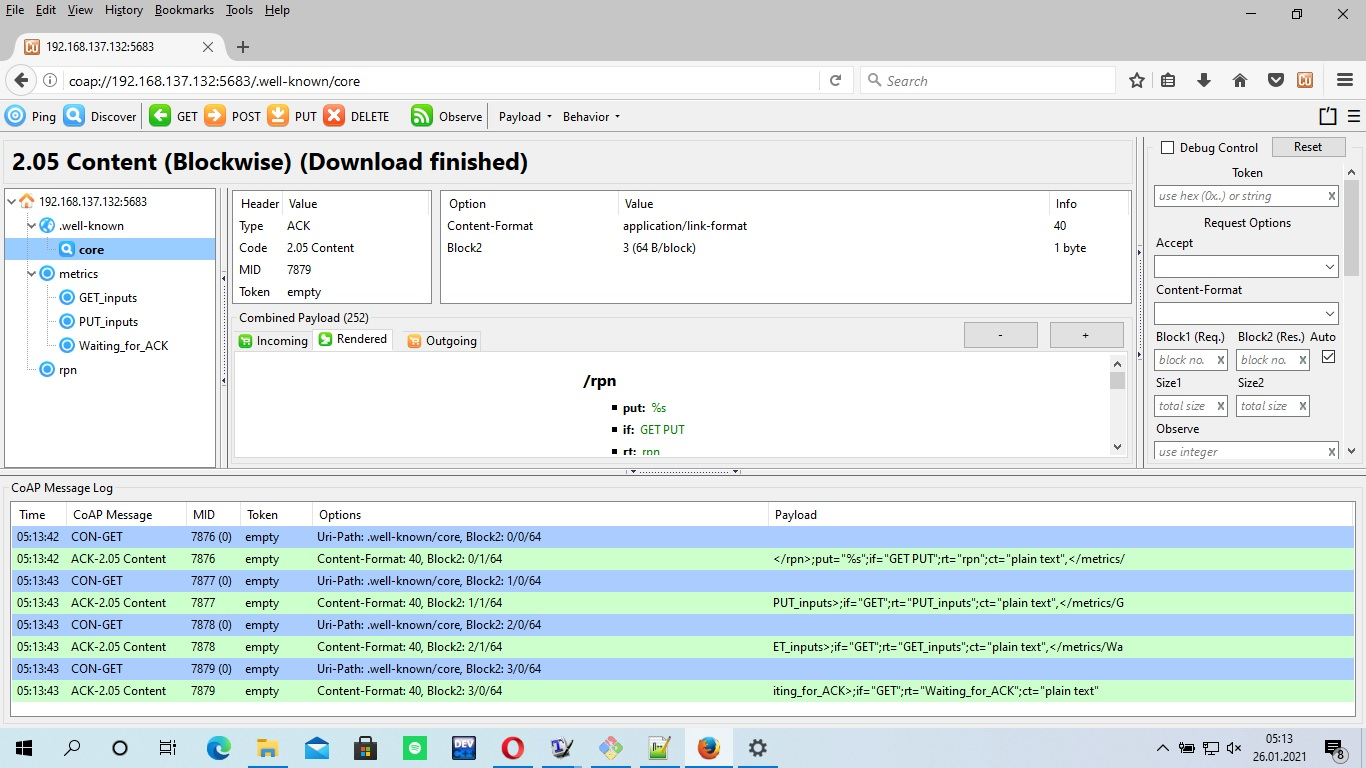
\includegraphics[scale=0.5]{img/well_known.jpg}
\end{figure}
\vspace{0.5cm}

Jak widzimy, zasób ten wysyła do klienta dane o wszystkich pozostałych zasobach.

\subsubsection{Zasób RPN}

\begin{enumerate}
\item  PUT

Kolejna linia rozpoczyna testowanie zasobu \textit{rpn}. Na początku wpisujemy dane wyrażenie. Rezultat wygląda następująco:

\begin{figure}[h]
    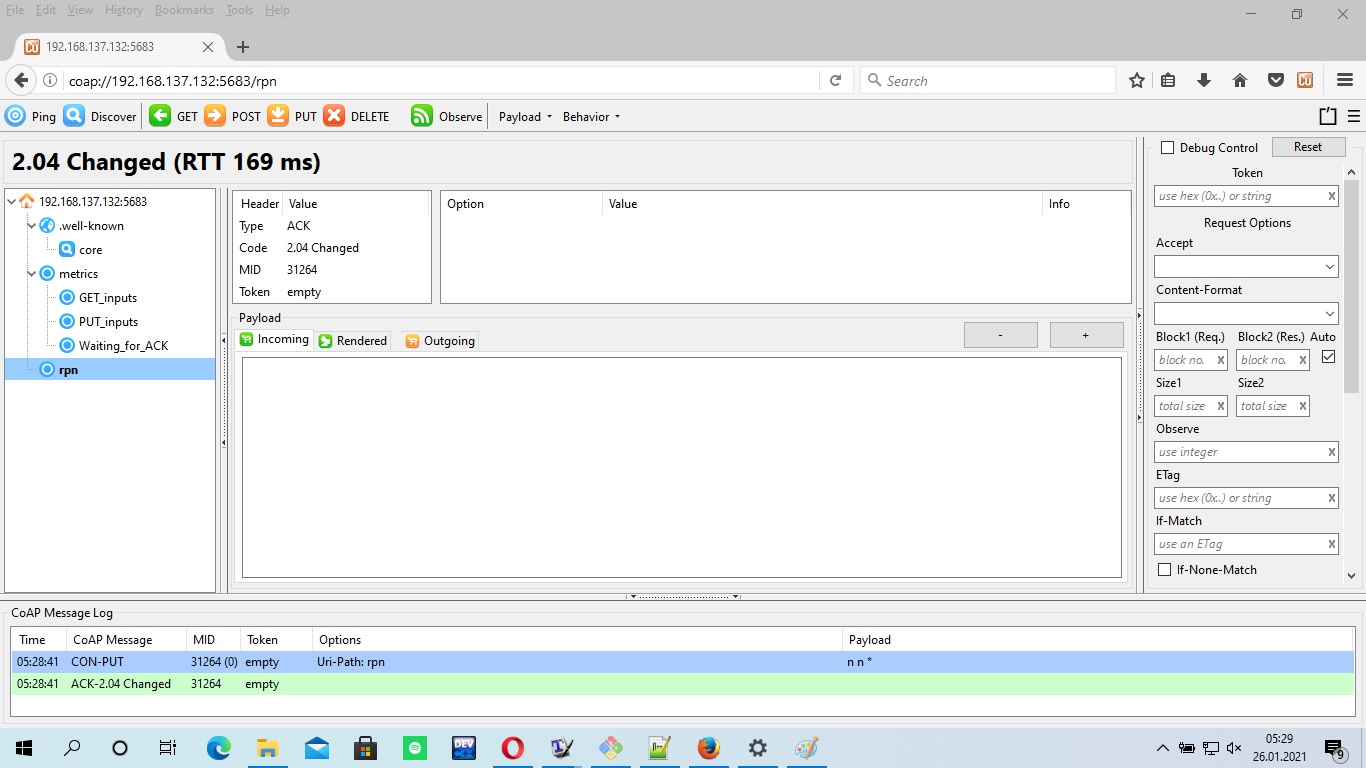
\includegraphics[scale=0.4]{img/rpn_put.jpg}
\end{figure}
\vspace{0.5cm}

Dana została pobrana i otrzymaliśmy potwierdzenie.

\item GET: pobranie wyniku

Teraz to wyrażenie, które wprowadziliśmy, obliczamy. Wynik mamy taki:

\begin{figure}[h]
    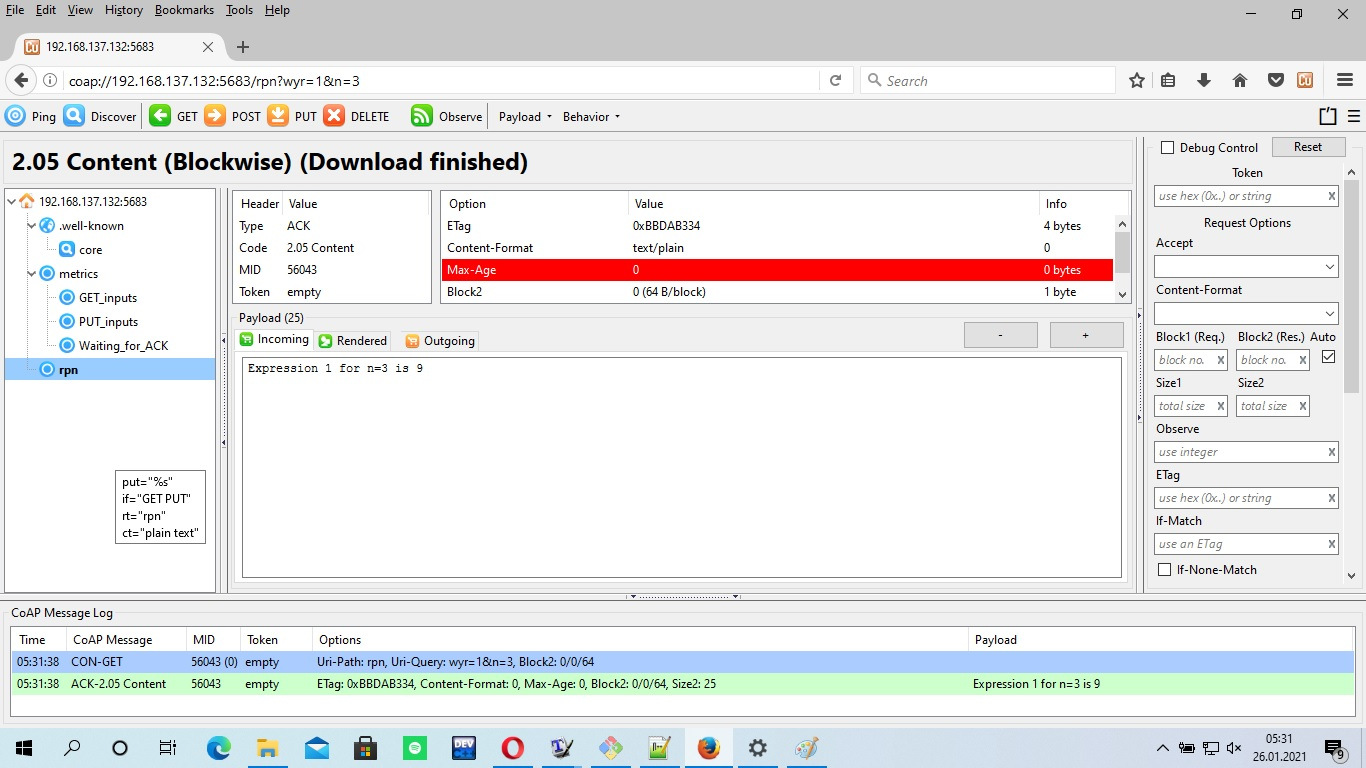
\includegraphics[scale=0.4]{img/rpn_get_wynik.jpg}
\end{figure}
\vspace{0.5cm}

Wynik został pobrany, jest on prawidłowy.

\item PUT: wpisanie dużej ilości wyrażeń

Następnym krokiem jest pętla, która przesyła kolejne wyrażenia przekraczając limit (u nas 10 wyrażeń). Wynik tej pętli jest następujący:

\begin{figure}[h]
    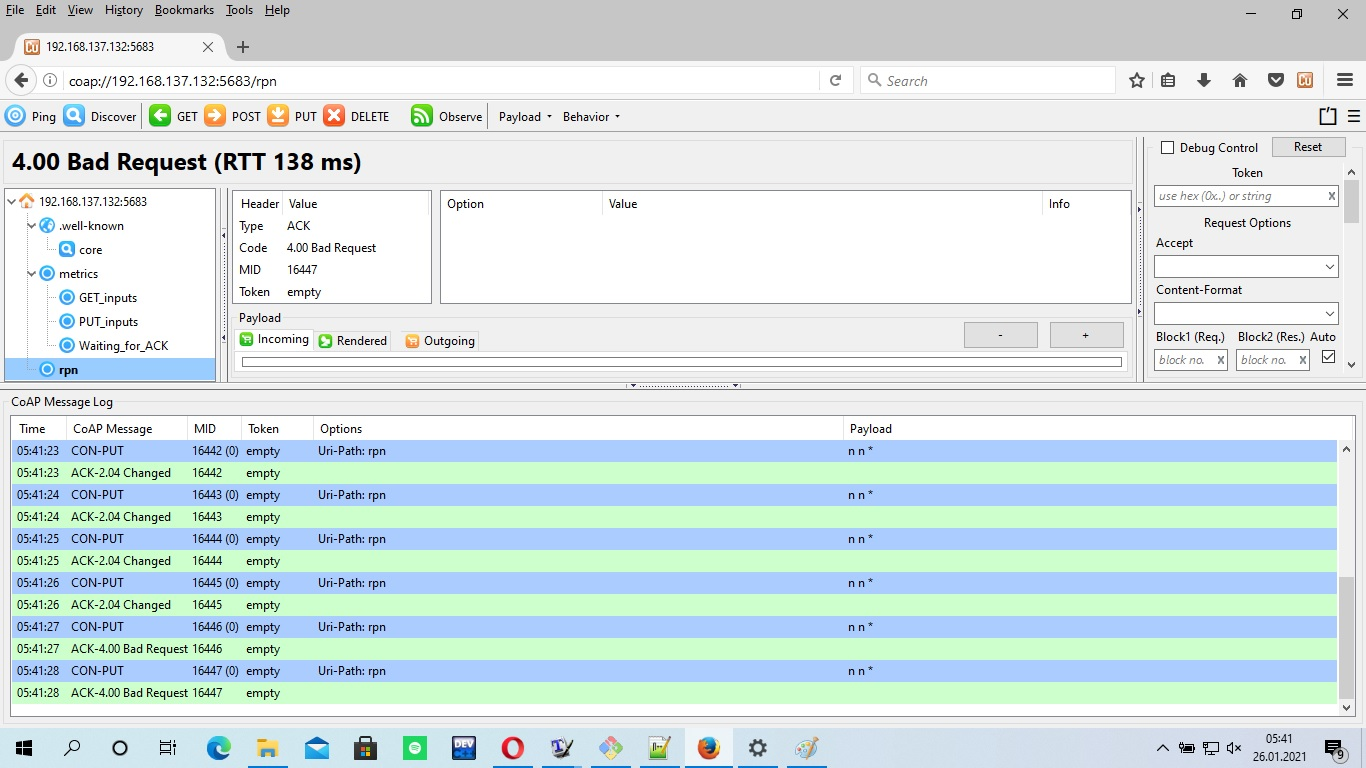
\includegraphics[scale=0.4]{img/rpn_put_duza_ilosc.jpg}
\end{figure}
\vspace{0.5cm}

Jak widzimy, po przekroczeniu danego limitu dostajemy wiadomości zwrotnie o kodzie 400 (Bad Request). To znaczy, że nasze ograniczenie wpisania zbyt dużej ilości danych działa.

\item GET: pobranie wyrażeń

Teraz wypiszemy nasze wyrażenia:

\begin{figure}[h]
    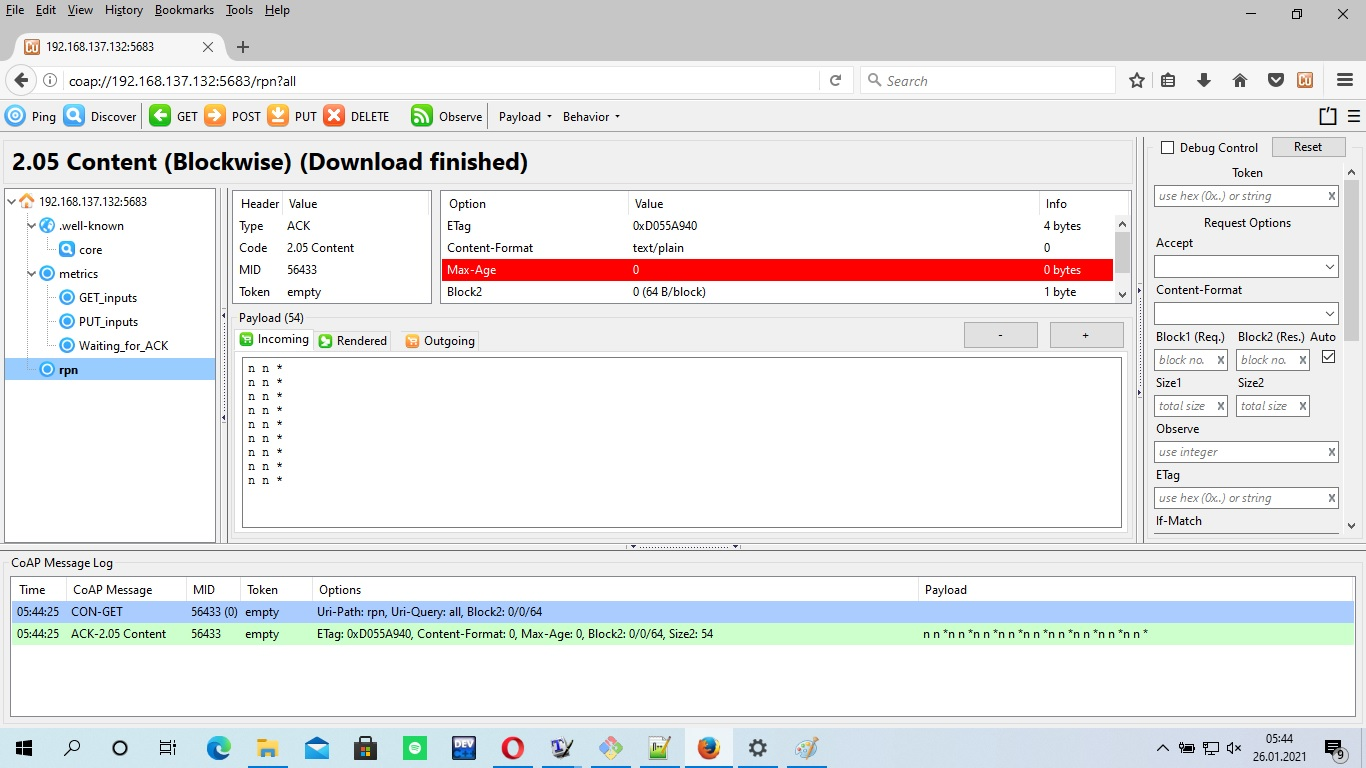
\includegraphics[scale=0.4]{img/rpn_get_all.jpg}
\end{figure}
\vspace{0.5cm}

Została nam zwrócona cała tablica wyrażeń, które poprzednio wpisaliśmy. Liczba ich jest 10.
\end{enumerate}

Tym przykładem kończymy testowanie zasobu RPN.

\subsubsection{Metryki}

W tym podrozdziale będziemy testować metryki.


\begin{enumerate}

\item GET\_inputs

Na sam początek sprawdzimy działanie zasobu GET\_inputs.

\begin{figure}[h]
    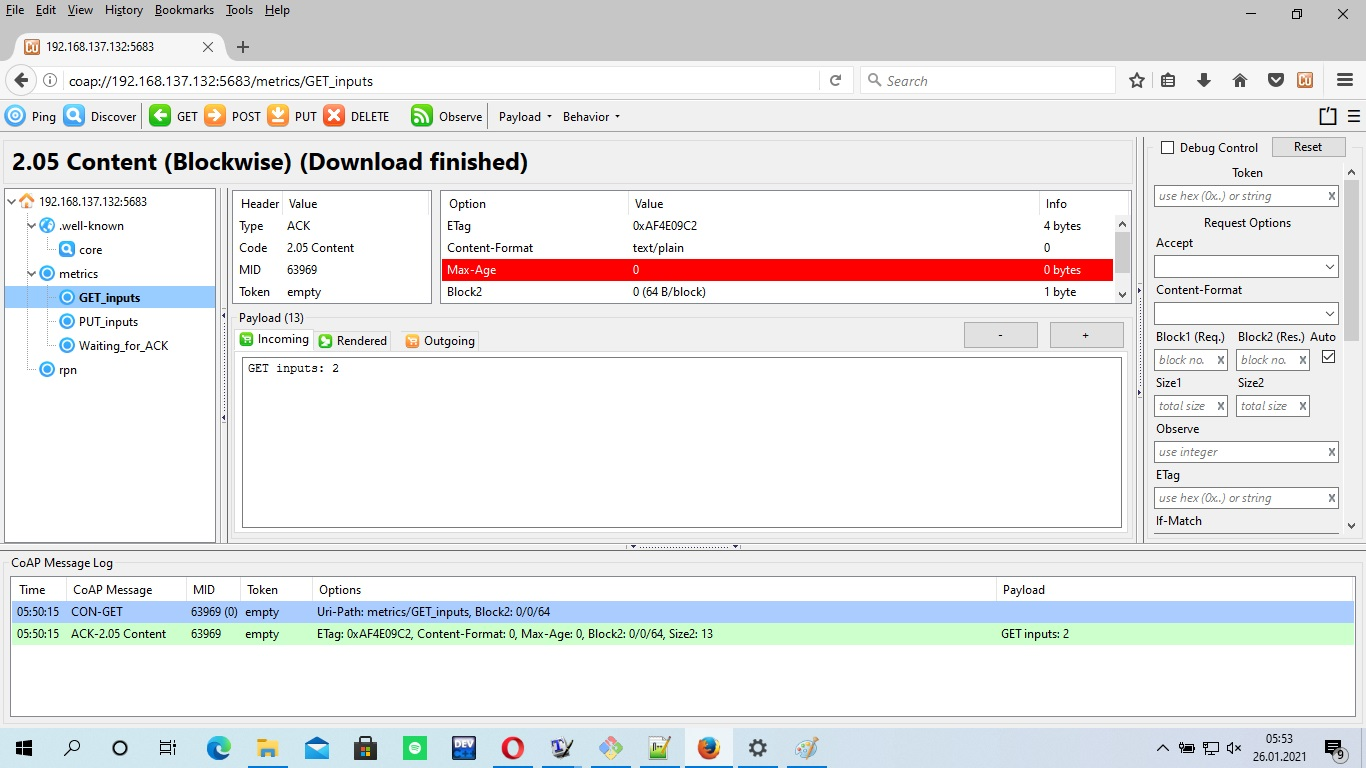
\includegraphics[scale=0.4]{img/met_get_inputs.jpg}
\end{figure}
\vspace{0.5cm}

Jak widzimy, została pobrana liczba odebranych żądań GET.

\item PUT\_inputs

Teraz sprawdzimy działanie zasobu GET\_inputs. Należy pamiętać, że ten zasób zwraca wiadomości CON oraz jest w trakcie jego obsługi włączony tryb "gubienia" wysyłanych datagramów.

\begin{figure}[h]
    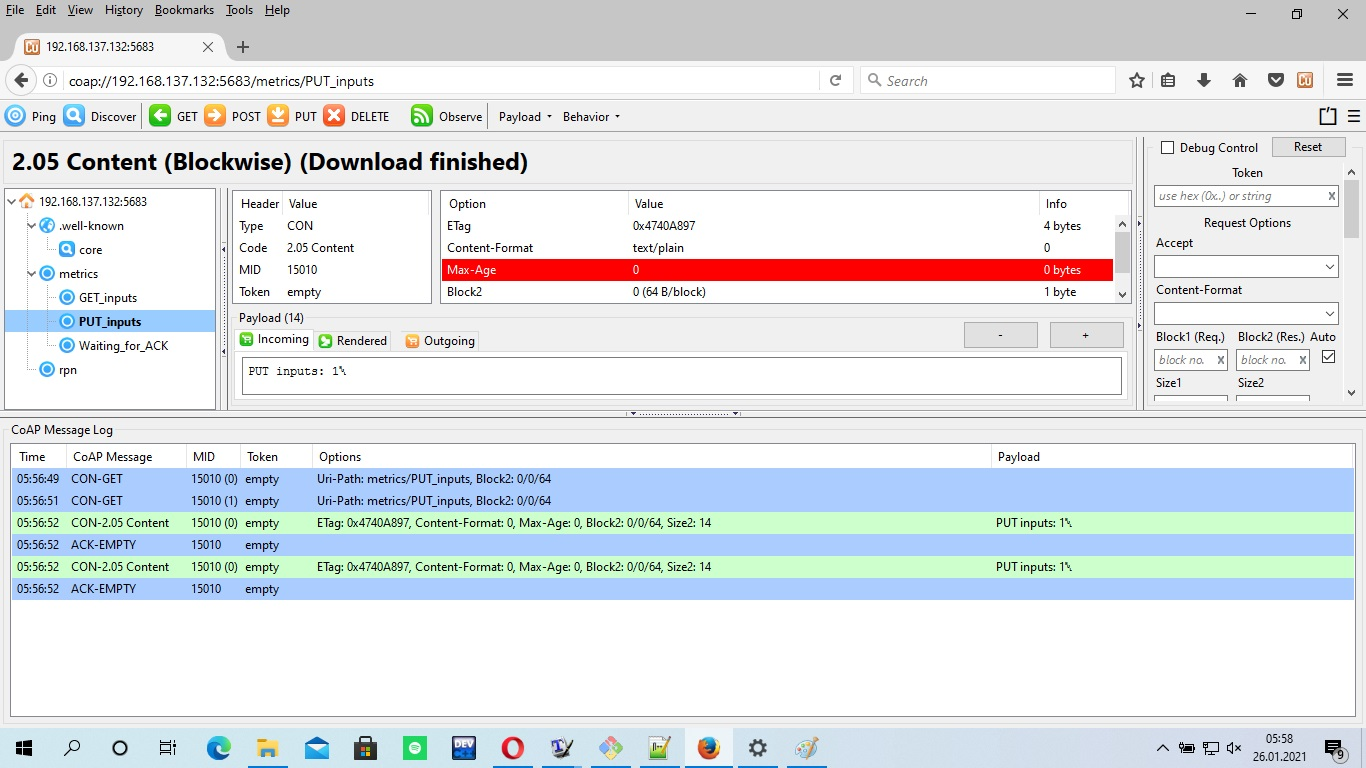
\includegraphics[scale=0.4]{img/met_put_inputs.jpg}
\end{figure}
\vspace{0.5cm}

Możemy zauważyć, że klient nie dostał za pierwszym razem odpowiedzi, więc ponawia wysłanie żądania. Lecz potem serwer odpowiada 2 razy, za każdym razem dostając od klienta potwierdzenie.

\item Waiting\_for\_ACK

Ostatnim zasobem, który będziemy testowac jest Waiting\_for\_ACK. Ten zasób natomiast jest zasobem o długim czasie dostępu, co będziemy mogli zaobserwować poniżej.

\begin{figure}[h]
    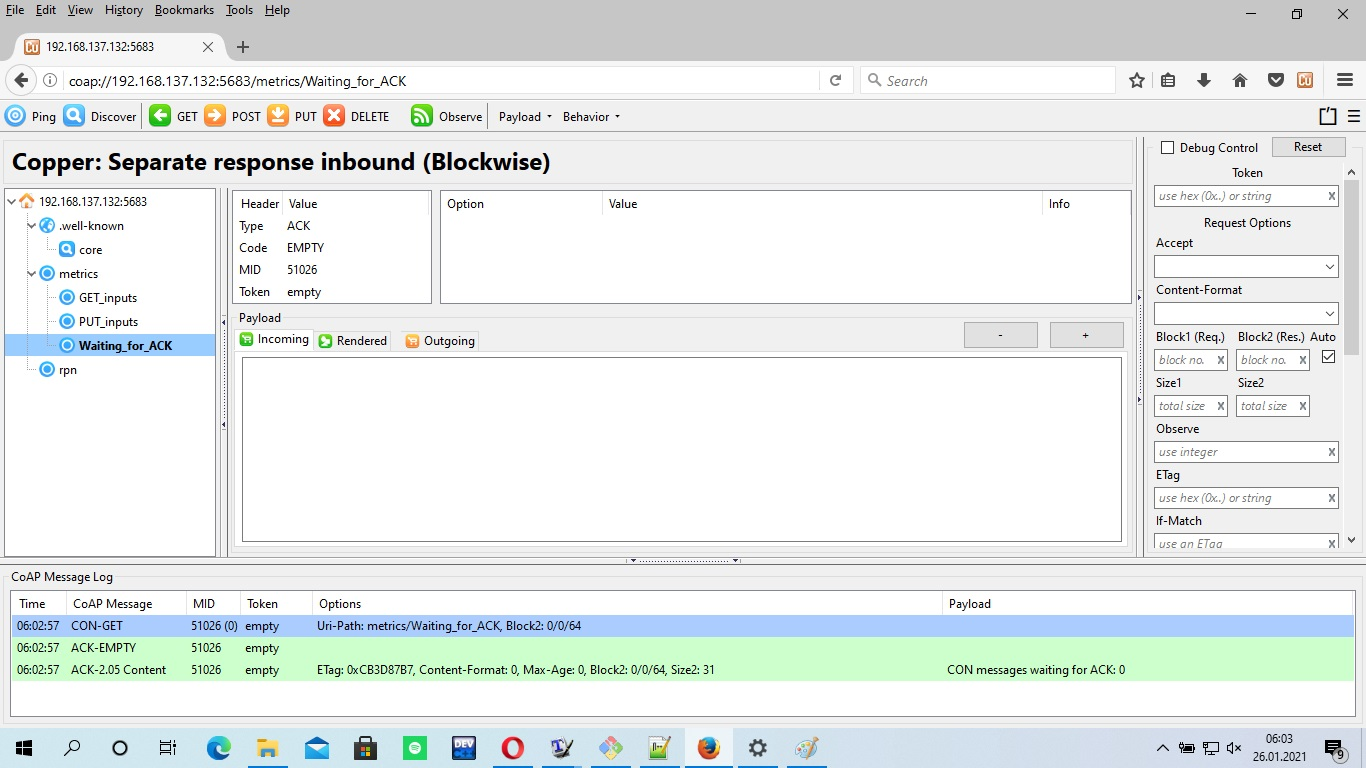
\includegraphics[scale=0.4]{img/met_ack.jpg}
\end{figure}
\vspace{0.5cm}

Jak widzimy, serwer od razu odpowiada odpowiedzią ACK, by dopiero potem wysłać odpowiedź na żądanie.
\end{enumerate}

\subsection {Testy - podsumowanie}

Dzięki poleceniom zawartym w skrypcie i scenariuszu testowania mogliśmy stwierdzić, że nasz serwer spełnia wymagania zadania.